\documentclass[10pt,border=2pt]{standalone}
\usepackage[T1]{fontenc}
\usepackage{lmodern}
\usepackage{pgfplots}
\pgfplotsset{compat=1.18}
\definecolor{convexblue}{HTML}{0072B2}
\definecolor{concaveorange}{HTML}{D55E00}
\begin{document}
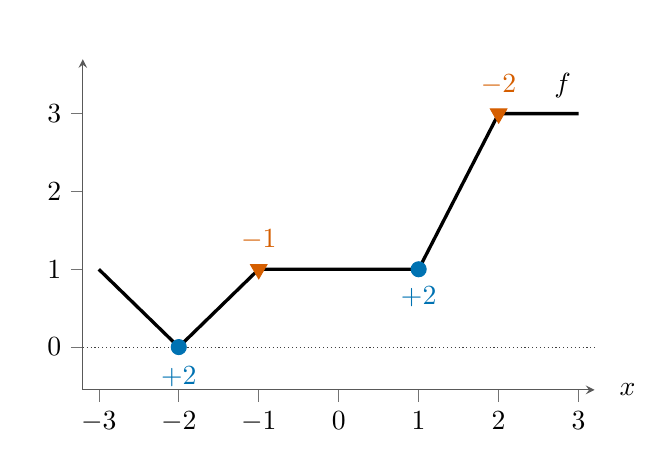
\begin{tikzpicture}
\path[use as bounding box] (-0.7,-0.65) rectangle (7.1,4.6);
\pgfplotsset{foldaxis/.style={
  scale only axis,width=6.5cm,height=4.2cm,
  at={(0,0)},anchor=south west,
  xmin=-3.2,xmax=3.2,xtick={-3,-2,-1,0,1,2,3},
  axis lines=left,axis line style={black!65},
  tick align=outside,tick style={black!55},
  xlabel={$x$},xlabel style={at={(axis description cs:1.03,0)},anchor=west},
  label style={font=\normalsize},tick label style={font=\normalsize},
  clip=false,
}}
\begin{axis}[foldaxis,ymin=-0.55,ymax=3.7,ytick={0,1,2,3}]
\addplot[black!75,densely dotted,thin] coordinates {(-3.2,0) (3.2,0)};
\addplot[black,very thick] coordinates {(-3,1) (-2,0) (-1,1) (1,1) (2,3) (3,3)};
\addplot[only marks,mark=*,mark size=2.7pt,convexblue] coordinates {(-2,0) (1,1)};
\addplot[only marks,mark=triangle*,mark options={rotate=180},mark size=3.4pt,concaveorange]
  coordinates {(-1,1) (2,3)};
\node[anchor=south] at (axis cs:2.8,3.08) {$f$};
\node[convexblue,anchor=north] at (axis cs:-2,-0.12) {$+2$};
\node[convexblue,anchor=north] at (axis cs:1,0.9) {$+2$};
\node[concaveorange,anchor=south] at (axis cs:-1,1.12) {$-1$};
\node[concaveorange,anchor=south] at (axis cs:2,3.12) {$-2$};
\end{axis}
\end{tikzpicture}
\end{document}
